\documentclass[11pt]{article}
\usepackage{aahomework}
\usepackage{mathtools}
\usepackage{subcaption}
\usepackage{epstopdf}
\usepackage{float}
\usepackage{xcolor}
\usepackage{parskip}
%\tikzstyle{blk}=[circle,inner sep=0pt,minimum size =4pt,draw,fill=black,line width=0.8pt]
%\tikzstyle{blanknode}=[circle,inner sep=3pt,minimum size =8pt,draw,line width=0.8pt]
%\tikzstyle{blk}=[circle,inner sep=0pt,minimum size =4pt,draw,fill=black,line width=0.8pt]
%
%\geometry{letterpaper, textwidth=17cm, textheight=22cm}

%\usetikzlibrary{arrows}
%\usetikzlibrary{plotmarks}

\newcommand{\ques}{\paragraph{Question:}}
\newcommand{\keyphrase}{\textbf}

\title{Lecture 2}
\author{A. Agarwal}
\date{December 7, 2012}


\begin{document}
%\maketitle

\section*{Recall}
\begin{enumerate}
\item{
System of linear equations.
}
\item{
Number of solutions of a system.
}
\item{
Row picture and column picture.
}
\end{enumerate}

\section*{New Terminology}
Two terms characterize the number of solutions to an equation:

\keyphrase{Consistent systems} have at least one solution. This could mean the system has one solution or infinitely many solutions.

\keyphrase{Inconsistent systems} have no solution.


Consider a system of equations:
\begin{align*}
\left.
\begin{aligned}
x + 3y &= 4
\\
5x - 4y &= -7
\end{aligned}
\right\}
\end{align*}
For such a system, we established that we can create an augmented matrix that represents it. The augmented matrix is made up of a coefficient matrix and a constant vector:
\begin{align*}
\left[
\begin{matrix}
1 & 3 & 4
\\
5 & -4 & -7
\end{matrix}
\right]
\end{align*}

Given an augmented matrix, we wish to reduce it to a `nice' form.
\begin{align*}
\left[
\begin{matrix}
1 & 3 & 4
\\
5 & -4 & -7
\end{matrix}
\right]
\xrightarrow[\text{to a nice form}]{\text{reduce this}}
\left[
\begin{matrix}
1 & 0 & *
\\
0 & 1 & *
\end{matrix}
\right]
\end{align*}
From this `nice' form of the augmented matrix, we can get the solutions of the system fairly easily. This will also tell us whether the system is consistent or inconsistent.

A good question is whether or not it is always possible for any augmented matrix to reduce the matrix to this type of form.

\section*{Row-operations}
\keyphrase{Row-operations} or elementary row operations allow us \emph{reduce} a matrix to achieve the matrix form that we want.
\begin{enumerate}
\item{
Swap rows
}
\item{
Multiply one row by a non-zero scalar
}
\item{
Adding a multiple of one row to another row
}
\end{enumerate}
It is not immediately clear why these operations are the important ones or why we are focusing on them. To understand these operations, we will consider again some system of equations. The key to row-operations is that they do not alter the solutions to a system of equations.

The first row operation is swapping the order of the equations. It is fairly intuitive that swapping the order of the equations will not change the solutions.

What about multiplication by a scalar? Consider the two systems below, where the second is obtained by multiplying the first equation by $2$:

\begin{align*}
\left.
\begin{aligned}
x + 3y &= 4
\\
5x - 4y &= -7
\end{aligned}
\right\}
\Longrightarrow
\left.
\begin{aligned}
2x + 6y &= 8
\\
5x - 4y &= -7
\end{aligned}
\right\}
\end{align*}

Next consider the third operation: adding a multiple of one row to another row. Of the operations, it is least obvious why this one does not alter the solutions of the system. In essence this operation is the addition a multiple of one equation to another equation. Consider within the example, adding negative-five times the first equation to the second equation:
\begin{align*}
\begin{aligned}
\left[\text{equation 1}\right]
\\
\left[\text{equation 1}\right] (-5) + \left[\text{equation 2}\right]
\end{aligned}
&&
\longrightarrow
&&
\begin{aligned}
x + 3y &= 4
\\
-19y &= -27
\end{aligned}
\end{align*}

\ques Will the solution set of the new system be the same as the solution set of the old system?

We can interpret this geometrically: each equation represents a line which we can plot.
\begin{figure}[H]
\centering
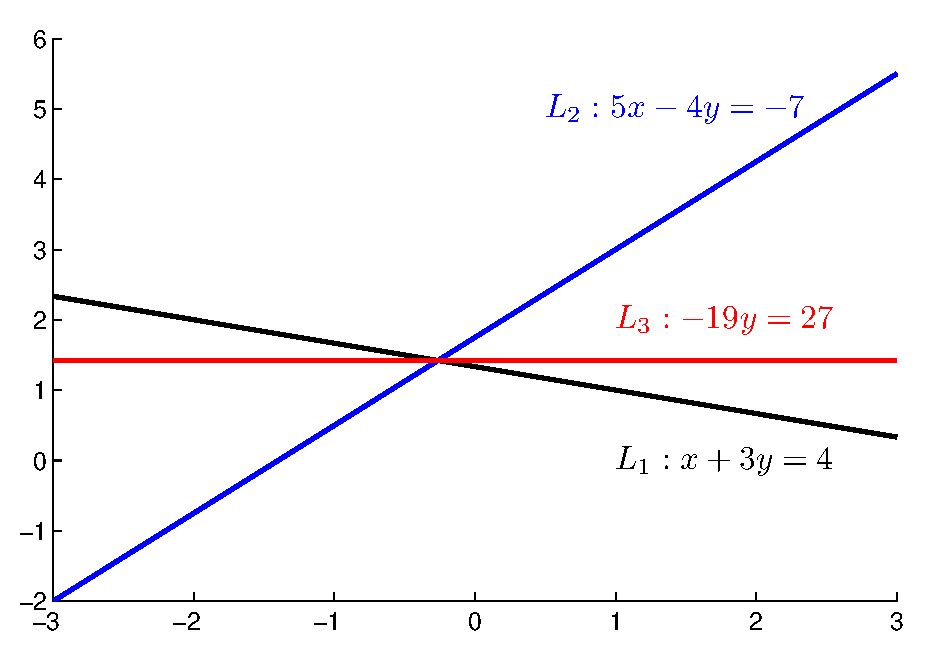
\includegraphics[width=10cm]{rowop3_visual.eps}
\end{figure}
It turns out that the line $L_3$ will intersect the first two lines at the mutual solution of those lines.

To interpret this algebraically, we can consider \emph{adding} the lines. The line $L_3$ was obtained by adding $L_2$ to $-5$ times $L_1$:
\begin{align*}
L_3 &= -5 L_1 + L_2
\end{align*}
If we consider replacing the expression ``$L_1$" by the equation $x+3y-4$ which algebraically represents it, and doing the same for $L_2$, then we obtain the following:
\begin{align*}
L_3 &= -5 L_1 + L_2
\\
&= -5(x+3y-4) + (5x-4y+7)
\end{align*}
Whenever the expression $x+3y-4$ is zero, then the point $(x,y)$ is on the line $L_1$, and similarly for $L_2$. Combining the two expressions, we arrive at an expression that will be zero only when the point lies on \emph{both} lines.
\begin{align*}
L_3 &= -5 L_1 + L_2
\\
&= -5(x+3y-4) + (5x-4y+7)
\\
&= -19y + 27
\end{align*}

That is, if a point $P = (x,y)$ is a solution to both lines $L_1$ and $L_2$, then it must be a solution to the line $L_3$:
\begin{align*}
-5(\underbrace{x+3y-4}_{\textcolor{red}{=0}}) + (\underbrace{5x-4y+7}_{\textcolor{red}{=0}})
=
\underbrace{-19y + 27}_{\textcolor{red}{\Rightarrow \hspace{.8cm} =0 \hspace{.8cm}\hphantom{\Rightarrow}}}
\end{align*}

\section*{Echelon form of a matrix}
The nice matrix forms that we want come in two forms. The first is \keyphrase{echelon form}.

\begin{minipage}[t]{.95\textwidth}
A matrix $M$ is in echelon form if
\begin{enumerate}
\item{
All the zero rows are at the bottom.
}
\item{
The leading non-zero entry of each row is to the right of the leading non-zero entry of the row above it.
}
\end{enumerate}
\end{minipage}

\paragraph{Examples.}
Consider the following matrices
\begin{align*}
A &= \begin{bmatrix}
1 & 2 & 3
\\
0 & 0 & 0
\end{bmatrix}
&
B &= \begin{bmatrix}
1 & 2 & 3
\\
0 & 1 & 0
\\
0 & 1 & 0
\end{bmatrix}
&
C &= \begin{bmatrix}
1 & 0 & 0 & 0
\\
0 & 0 & 1 & 0
\\
0 & 0 & 0 & 7
\end{bmatrix}
\end{align*}
The matrix $A$ satisfies condition (1) and since the first row is the only one with a leading non-zero entry and there is no row above it, $A$ satisfies condition (2) as well.

Matrix $B$ has no zero rows, so it satisfies condition (1). We see however that the leading non-zero entry of the third row is not to the right of the leading non-zero entry of the second row; thus matrix $B$ does not satisfy condition (2).

Matrix $C$ satisfies condition (1) and (2), so it is in echelon form. We can see that the leading non-zero entries of each row are strictly to the right of the leading non-zero entry of the rows above it.

\section*{Row-reduced echelon form: (rref)}

\begin{minipage}[t]{.95\textwidth}
A matrix $M$ is in row-reduced echelon form (rref) if
\begin{enumerate}
\item{
$M$ is in echelon form
}
\item{
All the leading non-zero entries must be $1$.
}
\item{
All the other entries in the column with leading $1$ should be $0$.
}
\end{enumerate}
\end{minipage}


Consider again the matrices
\begin{align*}
A &= \begin{bmatrix}
1 & 2 & 3
\\
0 & 0 & 0
\end{bmatrix}
&
B &= \begin{bmatrix}
1 & 2 & 3
\\
0 & 1 & 0
\\
0 & 1 & 0
\end{bmatrix}
&
C &= \begin{bmatrix}
1 & 0 & 0 & 0
\\
0 & 0 & 1 & 0
\\
0 & 0 & 0 & 7
\end{bmatrix}
\end{align*}

$A$ is in echelon form, but is it in row-reduced echelon form? It is, because all leading non-zero entries are $1$, and the other entries in that column are $0$.

$B$ is not in echelon form, so it cannot be in row-reduced echelon form.

$C$ is in echelon form, but it has a leading non-zero entry that is $7$, which violates condition (2).

\begin{figure}
\centering
$$\begin{bmatrix}
1 & 2 & 3
\\
0 & 0 & 0
\end{bmatrix}$$
\caption{Echelon and rref.}
\end{figure}

\begin{figure}
\centering
$$\begin{bmatrix}
1 & 2 & 3
\\
0 & 1 & 0
\\
0 & 1 & 0
\end{bmatrix}$$
\caption{Not echelon.}
\end{figure}

\begin{figure}
\centering
$$\begin{bmatrix}
1 & 0 & 0 & 0
\\
0 & 0 & 1 & 0
\\
0 & 0 & 0 & 7
\end{bmatrix}$$
\caption{Echelon but not rref.}
\end{figure}

From a theoretical perspective, echelon form and row-reduced echelon form are not very different. We can obtain the same information from a matrix in echelon form that we can from a matrix in row-reduced echelon form. From a matrix in row-reduced echelon form, we can fairly easily obtain the solutions, but it requires more computation to get a matrix into this form. Obtaining a solution from a matrix in echelon form may require back substitution to obtain answers.

Given an augmented matrix, we wish to obtain its echelon form and row-reduced echelon form.


\end{document}
